\documentclass[border=10pt]{standalone}
\usepackage[svgnames]{xcolor}
\usepackage{amsmath}
\usepackage{pgfplots}
\pgfplotsset{compat=newest}
\usepackage[sfdefault]{FiraSans}
\usepackage{FiraMono}
\renewcommand*\familydefault{\sfdefault}
\begin{document}
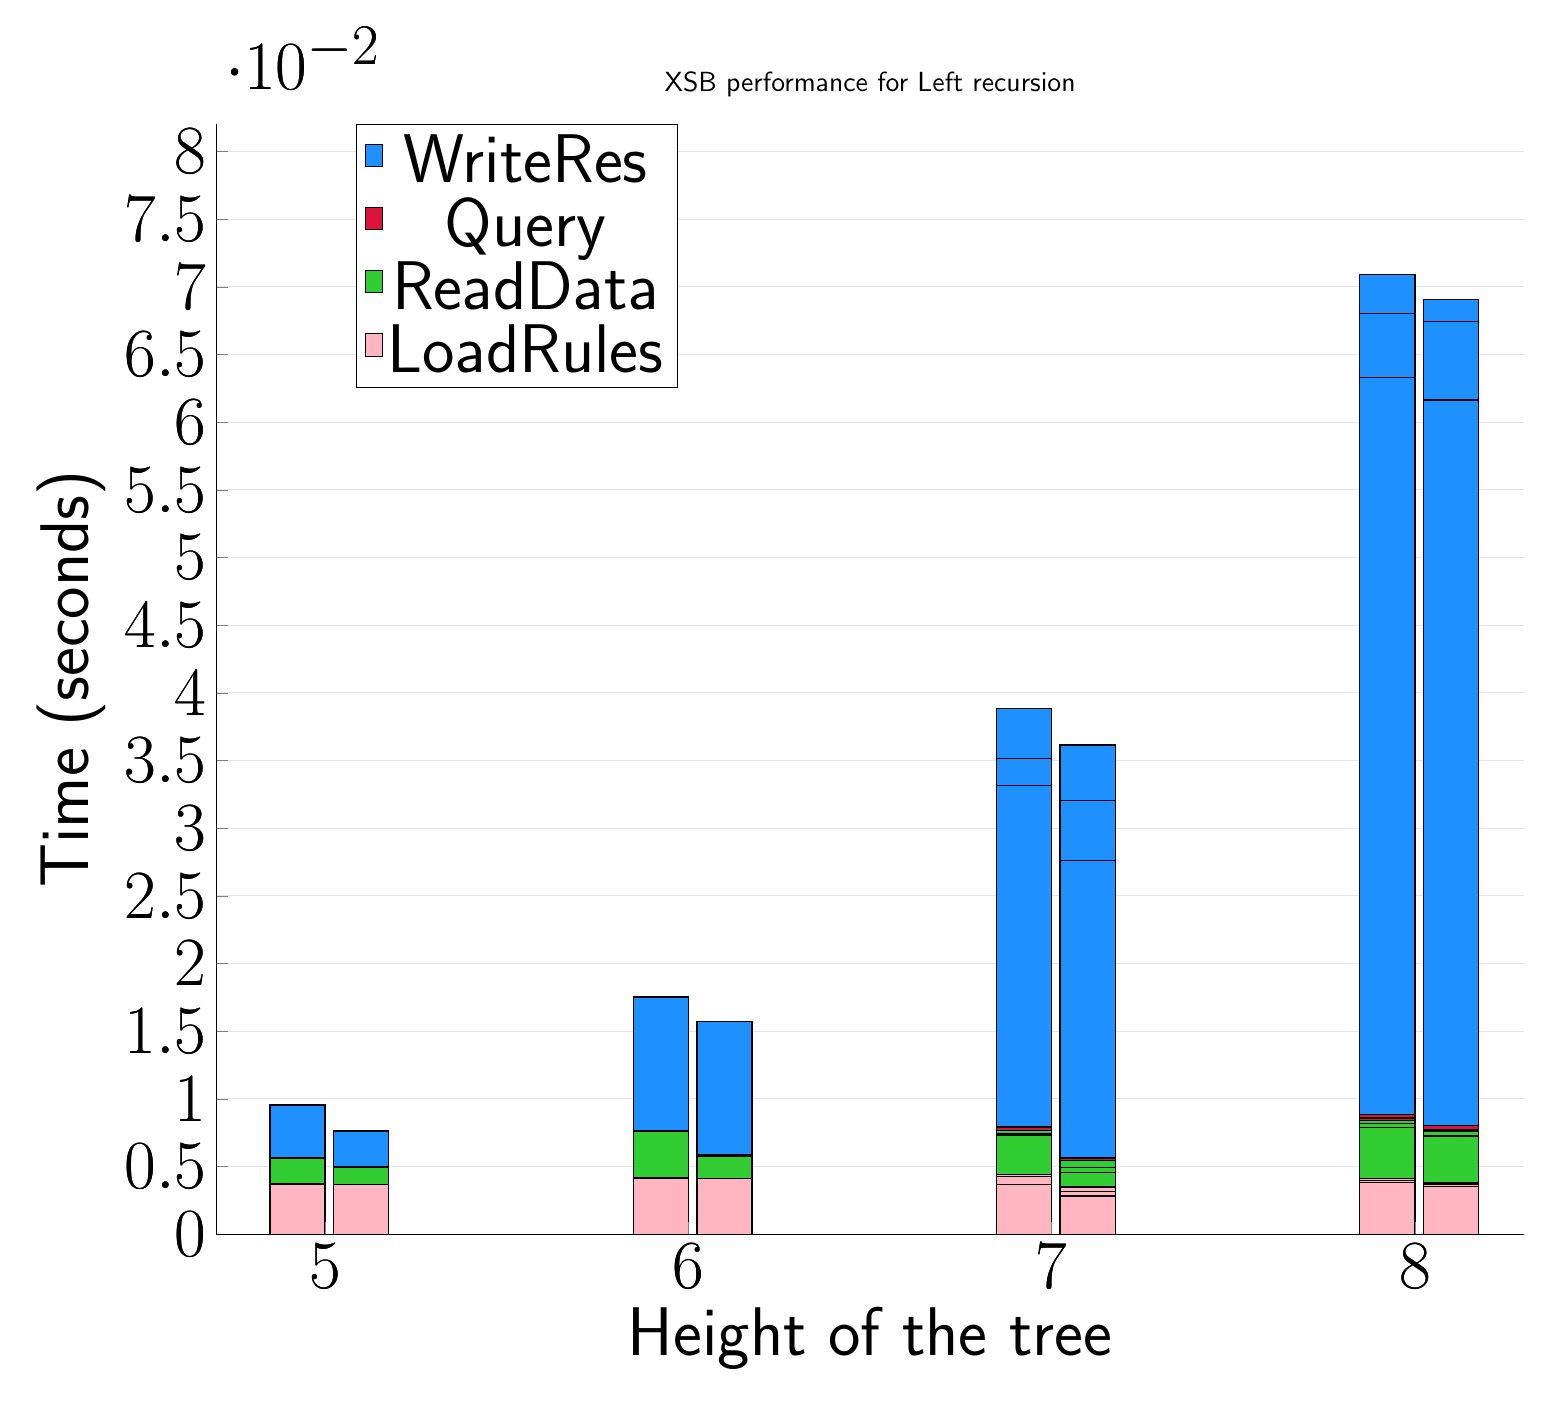
\begin{tikzpicture}
\begin{axis}[
   ybar stacked,
   title={XSB performance for Left recursion},
   bar shift=-10pt,
   width=1.5\textwidth,
   bar width=0.7cm,
   ymajorgrids, tick align=inside,
   major grid style={draw=gray!20},
   xtick=data,
   ymin=0, ymax=0.08207100550333658,
   axis x line*=bottom,
   axis y line*=left,
   enlarge x limits=0.1,
   legend style={
       at={(0.23, 1)},
       anchor=north,
       legend columns=1,
       font=\Huge,
   },
   ylabel={Time (seconds)},
   xlabel={Height of the tree},
   label style={font=\Huge},
   tick label style={font=\Huge},
]
\addlegendimage{fill=DodgerBlue, draw=black, line width=0.2pt}
\addlegendentry{WriteRes}
\addlegendimage{fill=Crimson, draw=black, line width=0.2pt}
\addlegendentry{Query}
\addlegendimage{fill=LimeGreen, draw=black, line width=0.2pt}
\addlegendentry{ReadData}
\addlegendimage{fill=LightPink, draw=black, line width=0.2pt}
\addlegendentry{LoadRules}
\addplot +[fill=LightPink, draw=black, line width=0.5pt] coordinates {
    (5, 0.0037096341451009133)
    (6, 0.004145304361979167)
    (7, 0.003684282302856443)
    (7, 0.00441130002339681)
    (7, 0.00428636868794759)
    (8, 0.00409833590189616)
    (8, 0.0039523442586263035)
    (8, 0.00382701555887858)
};
\addplot +[fill=LimeGreen, draw=black, line width=0.5pt] coordinates {
    (5, 0.00190099080403646)
    (6, 0.003447771072387693)
    (7, 0.0036516984303792293)
    (7, 0.003030697504679363)
    (7, 0.0033802986145019566)
    (8, 0.004317045211791993)
    (8, 0.003929932912190753)
    (8, 0.00435066223144531)
};
\addplot +[fill=Crimson, draw=black, line width=0.5pt] coordinates {
    (5, 4.46637471516927e-05)
    (6, 9.425481160481768e-05)
    (7, 0.0001773039499918617)
    (7, 0.00020662943522135435)
    (7, 0.00024843215942382796)
    (8, 0.0004233519236246746)
    (8, 0.0004467169443766273)
    (8, 0.0004185835520426433)
};
\addplot +[fill=DodgerBlue, draw=black, line width=0.5pt] coordinates {
    (5, 0.0038893222808837878)
    (6, 0.009854396184285496)
    (7, 0.02565677960713704)
    (7, 0.031214396158854175)
    (7, 0.027234951655069974)
    (8, 0.062071005503336586)
    (8, 0.05495699246724444)
    (8, 0.059424082438151025)
};
\end{axis}
\begin{axis}[
   ybar stacked,
   bar shift=13pt,
   width=1.5\textwidth,
   bar width=0.7cm,
   ymajorgrids, tick align=inside,
   major grid style={draw=none},
   xtick=data,
   ymin=0, ymax=0.08207100550333658,
   axis x line*=none,
   axis y line*=none,
   enlarge x limits=0.1,
   label style={font=\Huge},
   tick label style={font=\Huge},
]
\addplot +[fill=LightPink, draw=black, line width=0.5pt] coordinates {
    (5, 0.003689666666666666)
    (6, 0.004121333333333334)
    (7, 0.0031739999999999997)
    (7, 0.003501666666666667)
    (7, 0.0028339999999999997)
    (8, 0.003540666666666663)
    (8, 0.0037126666666666666)
    (8, 0.00379)
};
\addplot +[fill=LimeGreen, draw=black, line width=0.5pt] coordinates {
    (5, 0.0012596666666666635)
    (6, 0.001671333333333333)
    (7, 0.002276)
    (7, 0.0014449999999999999)
    (7, 0.001737)
    (8, 0.0040580000000000034)
    (8, 0.003551666666666667)
    (8, 0.0038436666666666667)
};
\addplot +[fill=Crimson, draw=black, line width=0.5pt] coordinates {
    (5, 4.433333333333373e-05)
    (6, 9.399999999999913e-05)
    (7, 0.000176666666666668)
    (7, 0.00010866666666666667)
    (7, 0.000234333333333334)
    (8, 0.0004226666666666663)
    (8, 0.0004459999999999996)
    (8, 0.00041833333333333333)
};
\addplot +[fill=DodgerBlue, draw=black, line width=0.5pt] coordinates {
    (5, 0.002643999999999999)
    (6, 0.009849666666666668)
    (7, 0.021969)
    (7, 0.031106666666666668)
    (7, 0.027242000000000002)
    (8, 0.061045999999999996)
    (8, 0.05393333333333333)
    (8, 0.05941133333333334)
};
\end{axis}
\end{tikzpicture}

\end{document}
